%%%%%%%%%%%%%%%%%%%%%%%%%%%%%%%%%%%%%%%%%%%%%%%%%%%%%%%%%%%%%%%%%%%%%%%%%%%%%%%%%%%%%%%%%%%
%                               My System 24pp
%%%%%%%%%%%%%%%%%%%%%%%%%%%%%%%%%%%%%%%%%%%%%%%%%%%%%%%%%%%%%%%%%%%%%%%%%%%%%%%%%%%%%%%%%%%
\chapter{Prototype}
\label{sec:implementation}

\section*{Summary}
A SleeveAR prototype was built to meet our vision expectations. To implement all planned features, our prototype had to rely on some already existing devices, mainly for motion tracking and feedback sources. This chapter will being with a description of our architecture and its most notable implementation details



\section{Architecture}
\label{sec:impl:arch}



\section{Tools}
\label{sec:impl:tools}

\subsection{Tracking Devices}


As for tracking devices, we had two different options to choose from.
The first makes use of the recently released, Microsoft Kinect One\footnote{\url{http://www.xbox.com/xboxone/kinect}} 
(previously baptized as Kinect 2), which supposedly offers a better tracking quality than 
the previous version, Kinect 1. Although this might be true, for our implementation we wanted a much more accurate and faster source of tracking, while also with a not so common tendency to fail due to camera occlusion.

The other alternative available at our laboratories was an OptiTrack Motion Capture system \footnote{\url{https://www.naturalpoint.com/optitrack/}}. 
This option offered us a more precise tracking and the possibility of dealing with occlusions due to the multiple cameras scattered around the room. 
The downside is the fact that it requires body markers to be used in order to successfully detect a person, unlike the 
Kinect which detects the human body through software algorithms. 
But using a comfortable and rather easy way to attach these body markers, made this not a bigger issue as it seems. 
A description of how we used the body markers can be found in section \ref{prototype-tracking}.



\subsection{Feedback Devices}

Providing feedback could be considered one of the foundations of this work. 
We chose to provide both visual and auditory feedback, being the latter much less vital to our goals in this implementation.

As it was described in section \ref{sec:sleevear}, our planned visual feedback would be applied on the user's arm and floor.
We relied on a light projector attached to the ceiling of our laboratory to project all visual feedback.
Details about how the light projections were able to hit the correct places, specifically the user's moving arm and floor, will be explained in section \ref{prototype-projection}.

Audio feedback was used simply to notify the user when to start the exercise and \todo{COMPLETAR}.
To provide audio, we relied on a speaker system also available at our laboratory

\subsection{Software}

We chose to implement our prototype with the well known \emph{Unity3D} game engine\footnote{\url{http://www.unity3d.com}}.
This engine already provides several tools that facilitate the development of augmented reality applications and we have in our possession already developed frameworks to communicate with the available tracking devices. In addition to this, Unity3D uses \texttt{C\#} as his main programming language, which is one of the most common languages use in the game development world, and already offers a wide range of solutions to create visual information.

\section{Setup Environment}
\todo{foto da sala}

All the work here presented was conducted in the Jo\~ao Louren\c{c}o Fernandes Laboratory, located at Campus Taguspark of T\'ecnico Lisboa, seen at figure \todo{figura}.
In this laboratory we had at our disposal all required devices to implement our work.

There were \todo{quantas camaras optitrack?} Optitrack motion sensors already fixed on the walls and prepared to use UDP communication to send tracking data. 
In section \ref{prototype-tracking} we will further explain the key points about our tracking system.
As for the light projector, a \todo{marca do projector} attached to the ceiling, as seen in figure \todo{figura do projector}, 
was used by connecting a VGA cable to our working computer.

\section{Implementation}

\subsection{Tracking}
\label{prototype-tracking}

As previously stated, we chose the Optitrack as our tracking system to implement SleeveAR's approach. This tracking system relies on body markers to capture movement.
These body markers are made of reflective material and are usually shaped as small spheres.

Optitrack is not able to track one single marker, instead, we need to use combinations of markers for it to calculate both position and rotation of the combination's center of mass. To create combinations, we used small plastic objects onto which was possible to attach several markers.

After combining at least three markers, they could be assigned an ID inside Optitrack software. 
From then on, the software was able to identify that specific combination and provide us with its current position and rotation.
For easier understanding, and writing, of this section, we will name this markers combination as a \textbf{rigid body}.

With this in mind, for our work, we required three different rigid bodies. Each one should be attached to a different arm location, in this case, shoulder, elbow and wrist. 
By doing so, we were able to receive tracking data from the three locations, and therefore, replicate the arm with data.

Our first method of placing the each rigid body was by using a Velcro bracelet around each location of the arm. Each rigid body would then be attached to each bracelet. This method didn't have a positive result for several reasons. First, it took to long to attach each bracelet around the arm, in addition, the Velcro material provoked discomfort when pressed hard against the skin. Second, the bracelets tended to move out of place, especially in the shoulder area where it was particularly hard to properly hold it in place.

Having an easy way to attach and hard to move method of holding our rigid bodies was vital for our work. Rigid bodies moving out of place during a movement could result in unwanted and unexpected results. Therefore, we created a better attachment method, by using a custom designed sleeve.


\subsubsection{Sleeve}

\begin{figure}[!t]
    \begin{center}
        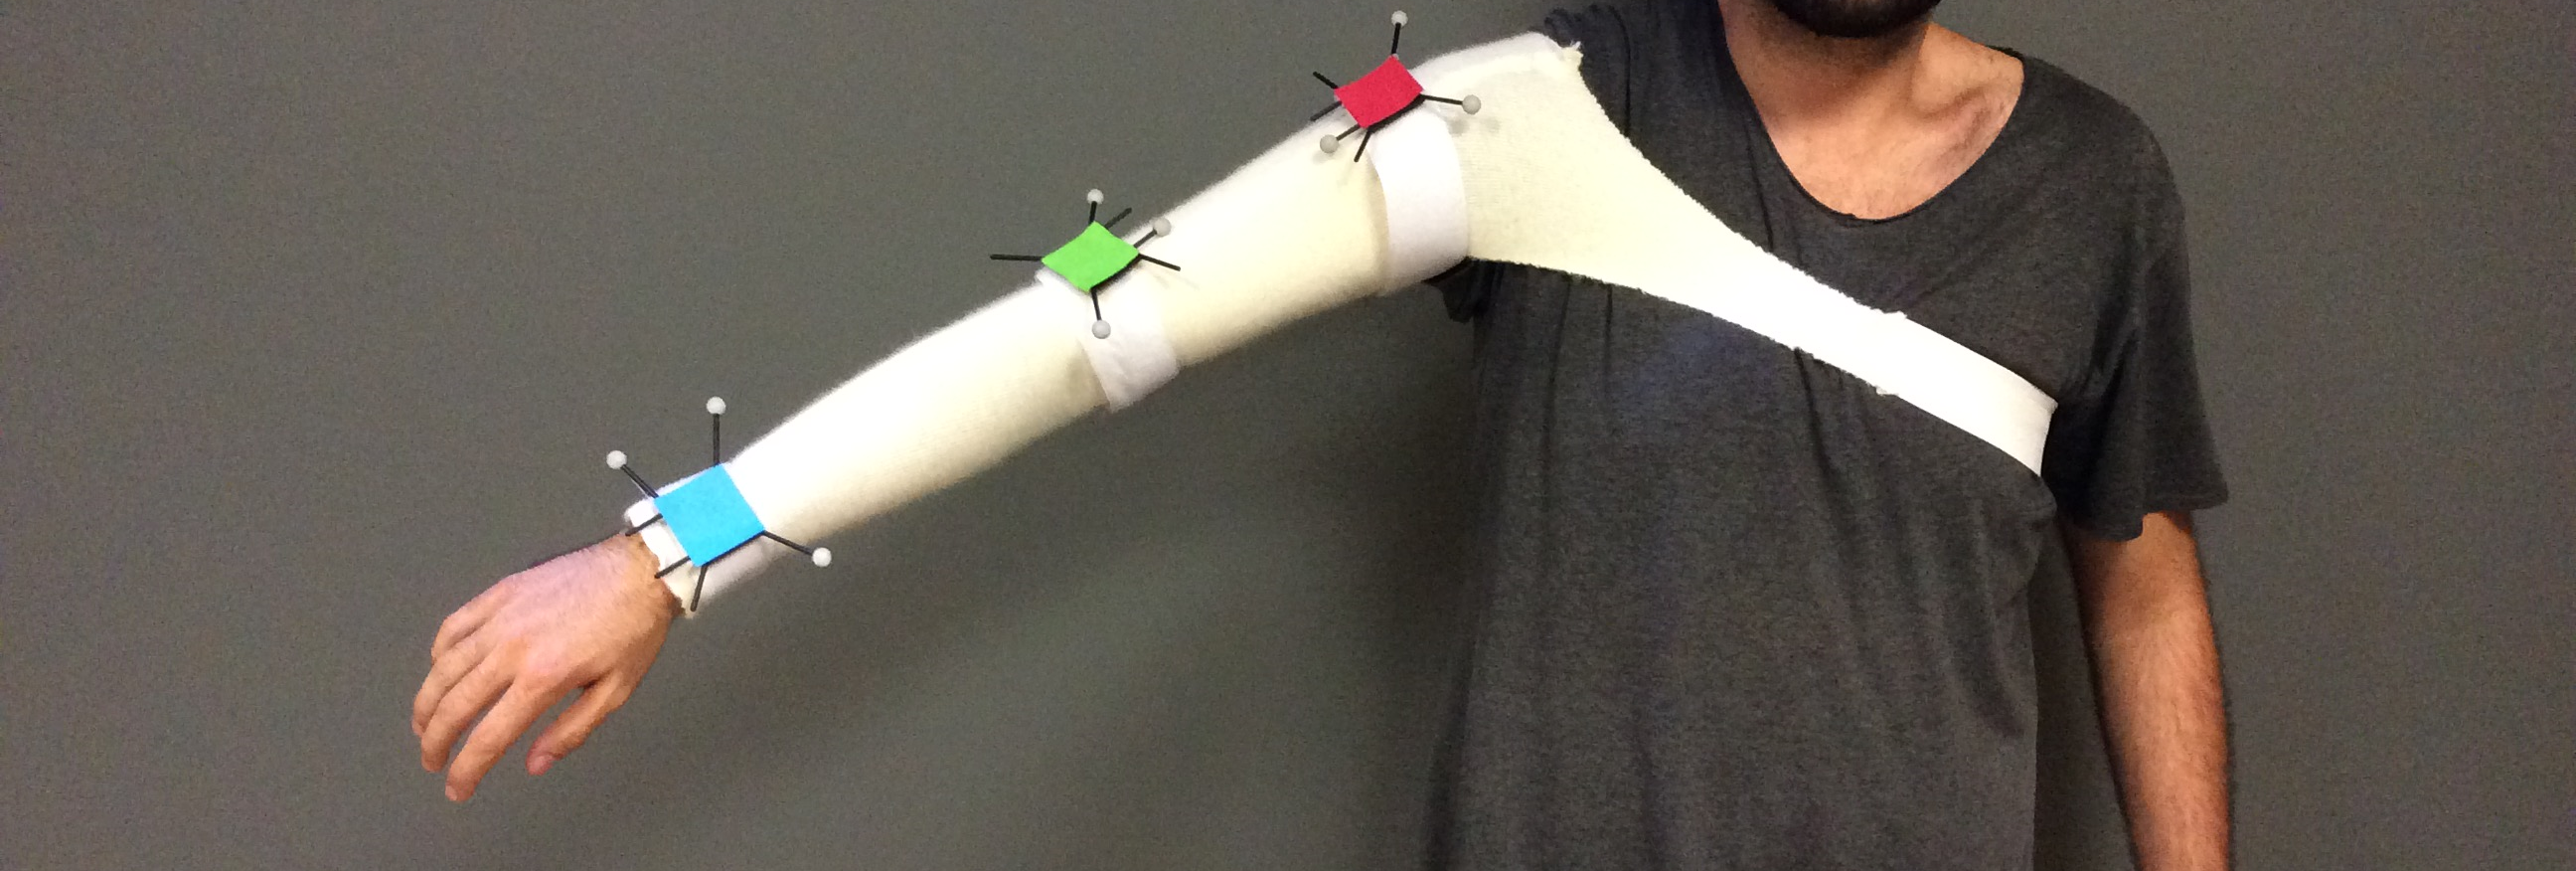
\includegraphics[width=\textwidth]{imgs/sleevewearable.png}
    \end{center}
    \caption{Sleeve used for tracking.}
    \label{fig:sleevewearable}
\end{figure}

We designed a custom sleeve, seen at figure \ref{fig:sleevewearable}, made out of wool material. This solved our previously presented problems by fixing the sleeve in place using a kind of "belt" around the user's torso which greatly increased its stability. Each of the rigidbodies were still attached to a bracelet, but in this case the bracelets were stitched to the sleeve. This improved significantly the rigid bodies attachment due to the bracelets never leaving the sleeve, while also enabling us to still squeeze them more or less depending on the user's arm thickness.

\todo{white because of the color projections}

\subsection{Projection}
\label{prototype-projection}

\todo{mais cenas}